
%\documentclass[10pt,twoside,twocolumn]{article}
\documentclass[12pt,twoside]{article}
\usepackage[bf,small]{caption}
\usepackage[letterpaper,hmargin=1in,vmargin=1in]{geometry}
\usepackage{paralist} % comapctitem, compactdesc, compactenum
\usepackage{titlesec}
\usepackage{titletoc}
\usepackage{times}
\usepackage{hyperref}
\usepackage{algorithmic}
\usepackage{graphicx}
\graphicspath{{./graphics/}}
\usepackage{xspace}
\usepackage{verbatim}
\usepackage{url}
\usepackage{float}
\hyphenation{Sub-Bytes Shift-Rows Mix-Col-umns Add-Round-Key}

\setlength{\parskip}{12pt}
\setlength{\parindent}{0pt}

\newcommand{\hdb}{\emph{hashdb}\xspace}
\newcommand{\bulk}{\emph{bulk\_extractor}\xspace}
\newcommand{\mdd}{\emph{md5deep}\xspace}
\newcommand{\bev}{\emph{Bulk Extractor Viewer}\xspace}

\begin{document}

\begin{center}
\Large Demo: Creating a Block Hash Database \\
\large Using \hdb and \mdd
\end{center}

We build large databases of block hashes
to help us find fragments of previously encountered data.
Here are some ways \hdb databases are used:
\begin{compactitem}
\item We scan data looking for block hashes that match
block hashes in previously encountered data.
\item We subtract data known to be not interesting, such as system files,
to remove distracting false positives.
\end{compactitem}
The Scanner demo at
\url{http://digitalcorpora.org/downloads/hashdb/demo/scanner\_demo.pdf}
uses a block hash database to find previously encountered data
in a media image.

The Similarity demo at
\url{http://digitalcorpora.org/downloads/hashdb/demo/similarity\_demo.pdf}
compares two block hash databases created from two media images to find 
fragments of user data that are common between them.

In this demo, we create block hash database \texttt{mock\_video.hdb}
of mock video file \texttt{mock\_video.mp4}
to use as a reference for finding previously encountered data.
The database we create is the very database we use in the
introductory demo for finding fragments of previously encontered data at
\url{http://digitalcorpora.org/downloads/hashdb/demo/scanner\_demo.pdf}.

Workflow:
\begin{compactenum}
\item Generate a DFXML file containing block hashes
from sources of ``previously encountered'' data.

\begin{figure}[H]
  \center
  
\includegraphics[scale=0.6]{drawings/md5deep}
  \caption*{Run \mdd to create a DFXML file of block hashes from your \\
            library of prevously encountered files.}
\end{figure}

\item Import the DFXML file of block hashes into a block hash database.

\begin{figure}[H]
  \center
  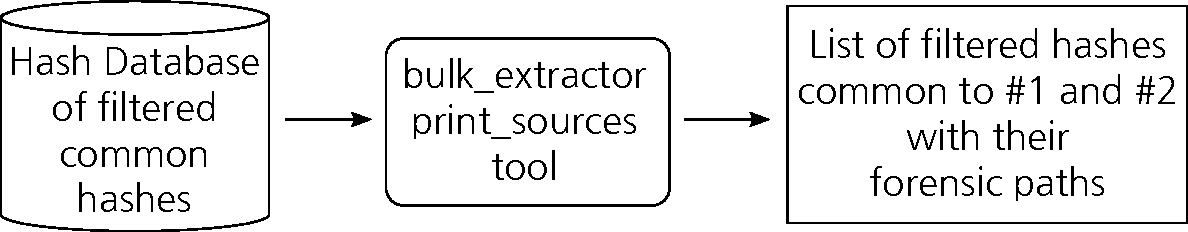
\includegraphics[scale=0.6]{drawings/import}
  \caption*{Run the \hdb \texttt{import} command
            to import block hashes into the hash database.}
\end{figure}

\end{compactenum}

Steps:
\begin{compactenum}
\item Download and install \hdb and \bulk compiled with the \hdb scanner
from
\url{http://digitalcorpora.org/downloads/hashdb}
as described in the Scanner demo
for finding part of a video file in a media image,
\url{http://digitalcorpora.org/downloads/hashdb/demo/scanner\_demo.pdf}
\item Pick a directory or file to use
as your source of files.
For this demo, please download and use the mock video file at
\url{http://digitalcorpora.org/downloads/hashdb/demo/mock\_video.mp4}.

\item Use the \mdd tool to generate the DFXML file of block hashes
of your files and directories:
\begin{compactitem}
\item Use \texttt{-p 4096} to specify a block (partition) size of 4096.
\item Use \texttt{-d} to generate output in DFXML format.
%\item Use \texttt{-r} to generate block hashes recursively in subdirectories.
\item Use \texttt{> mock\_video\_hashes.xml} to direct the DFXML output
to go to file \\
\texttt{mock\_video\_hashes.xml}.
\end{compactitem}
\begin{verbatim}
$ md5deep -p 4096 -d mock_video.mp4 > mock_video_hashes.xml
\end{verbatim}

\item Use the \hdb tool to \texttt{create} a new hash database
called \texttt{mock\_video.hdb}:
\begin{verbatim}
$ hashdb create mock_video.hdb
\end{verbatim}

\item Use the \hdb tool to \texttt{import} the block hashes
from the DFXML file into the new hash database:
\begin{verbatim}
$ hashdb import mock_video_hashes.xml mock_video.hdb
\end{verbatim}
\end{compactenum}

This completes the demo.

\end{document}

